
Istniejące algorytmu grupowania można podzielić ze względu na to jak definiują pojęcie grupy. Jedną z klas algorytmów grupowania są właśnie algorytmy grupowania gęstościowego. Jak wskazuje nazwa, grupy określa się na podstawie lokalnej gęstości punktów, co zgadza się z intuicyjnym pojęciem grupy.\par

Część algorytmów grupowania gęstościowego opiera się na dzieleniu przestrzeni na siatkę komórek, gdzie grupy określane są na podstawie uśrednionej gęstości wewnątrz tychże komórek. O ile takie podejście jest proste i wydajne, to nie jest dokładne, a wyniki grupowania mogą zależeć od rozmieszczenia siatki. Algorytm DBSCAN reprezentuje podejście, które rozwiązuje te problemy. Przynależność do grupy jest rozstrzygana dla każdego punktu oddzielnie, więc grupowanie jest dokładne co do punktu. Co więcej, wyniki są deterministyczne z dokładnością do tak zwanych punktów brzegowych.\par
Definicja grupy zaproponowana w DBSCAN okazała się na tyle skuteczna, że powstały liczne algorytmy pochodne opierające się na tej samej lub podobnej definicji grupy. Takimi algorytmami są SUBCLU oraz PREDECON. Obydwa należą do klasy algorytmów grupowania w podprzestrzeniach, co oznacza, że są w stanie wyznaczać grupy w podzbiorach atrybutów grupowanych obiektów.\par
W tym rozdziale zostaną przedstawione trzy wspomniane wcześniej algorytmy: DBSCAN, SUBCLU oraz PREDECON.

\section{DBSCAN}
DBSCAN jest popularnym algorytmem grupowania gęstościowego. Najważniejsze jego zalety wymienione w \cite{dbscan} to tworzenie grup o dowolnym kształcie oraz możliwość doboru parametrów przy niewielkiej wiedzy o zbiorze danych. Grupy tworzone są na podstawie lokalnej gęstości punktu rozumianej jako liczba punktów w otoczeniu punktu, dzięki czemu tworzone są grupy o intuicyjnych kształtach.

Zakładamy, że grupowany jest zbiór punktów $ D $. Na potrzebę algorytmu definiuje się pojęcie $ \varepsilon $-otoczenia punktu $ p \in D $. Jest to zbiór punktów znajdujących się w odległości nie większej niż punkt, dla którego jest wyznaczane otoczenie. Dalej $ \varepsilon $-otoczenie punktu $ p $ będzie oznaczane $ N_\varepsilon(p) $.
\begin{equation}\label{eps-neighbourhood}
	N_\varepsilon(p) = \set{q \in D | d(p, q) \le \varepsilon}
\end{equation}

Punkt, który posiada w swoim otoczeniu $ N_\varepsilon(p) $ conajmniej $ \mu $ punktów jest nazywany punktem rdzeniowym.
\begin{equation}\label{core-point}
	core_{\varepsilon,\mu}(p) \iff |N_\varepsilon(p)| \le \mu
\end{equation}
\begin{figure}
	\centering
  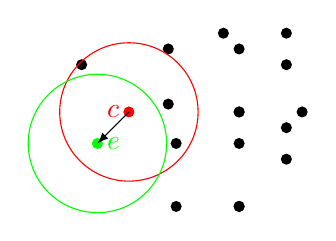
\begin{tikzpicture}
		\fill (-2,1.8) circle(2pt);
		\fill (-.9, 1.3) circle(2pt);
		\fill (-.9,2) circle(2pt);
		\fill (-.8,.8) circle(2pt);
		\fill (-.8,0) circle(2pt);
		\fill (-.2,2.2) circle(2pt);
		\fill (0,0) circle(2pt);
		\fill (0,1.2) circle(2pt);
		\fill (0,1.2) circle(2pt);
		\fill (0,0) circle(2pt);
		\fill (0,.8) circle(2pt);
		\fill (0,2) circle(2pt);
		\fill (.6,1) circle(2pt);
		\fill (.6,.6) circle(2pt);
		\fill (.6,1.8) circle(2pt);
		\fill (.6,2.2) circle(2pt);
		\fill (.8,1.2) circle(2pt);
    
    \fill[red] (-1.4,1.2) circle(2pt) node[anchor=east]{$ c $};
    \draw[red] (-1.4,1.2) circle(25pt);
    
    \fill[green] (-1.8,.8) circle(2pt) node[anchor=west]{$ e $};
    \draw[green] (-1.8,.8) circle(25pt);
    
		\draw[-latex] (-1.4,1.2) -- (-1.8,.8);
		
  \end{tikzpicture}
  \caption{Punkt rdzeniowy $ c $, brzegowy $ e $ oraz relacja bezpośredniej gęstościowej osiągalności $ dirreach_{\varepsilon,\mu}(e, c) $, $ \mu=3$.}\label{fig:core-edge-point}
\end{figure}

Dalej, na potrzebę definicji grupy wprowadza się pojęcie bezpośredniego zasięgu gęstościowego. Jest to niesymetryczna relacja, która zachodzi jeśli punkt znajduje się w $ \varepsilon $-otoczeniu punktu rdzeniowego. Punkt $ p $ jest w bezpośrednim zasięgu gęstościowym punktu $ q $, jeśli punkt $ q $ jest punktem rdzeniowym i $ p $ znajduje się w $ \varepsilon $-otoczeniu punktu $ q $.
\begin{equation} \label{direct-reachability}
	dirreach_{\varepsilon,\mu}(p, q) \iff p \in N_\varepsilon(q) \land core_{\varepsilon,\mu}(q)
\end{equation}
To, że $ p $ jest w bezpośrednim zasięgu gestościowym $ q $ nie determinuje, \mbox{że $ q $ jest} w bezpośrednim zasięgu gęstościowym $ p $.
\begin{equation} \label{direct-reachability-asymmetry}
	dirreach_{\varepsilon,\mu}(p, q) \centernot \implies dirreach_{\varepsilon,\mu}(q, p)
\end{equation}

Punkt, który jest w bezpośrednim zasięgu gęstościowym innego punktu, ale sam nie jest punktem rdzeniowym jest nazywany punktem brzegowym.
\begin{equation}\label{edge-point}
	edge_{\varepsilon,\mu}(p) \iff \neg core_{\varepsilon,\mu}(p) \land dirreach_{\varepsilon,\mu}(p,q)
\end{equation}

Jeśli punkt $ p $ jest w bezpośrednim zasięgu gęstościowym $ q $, to jest też w zasięgu gęstościowym $ q $. 
\begin{equation}
	dirreach_{\varepsilon,\mu}(p, q) \implies reach_{\varepsilon,\mu}(p, q)
\end{equation}
Zasięg gęstościowy jest relacją przechodnią, to znaczy, że jeśli $ p $ jest w zasięgu gęstościowym $ q $  i $ q $ jest w zasięgu gęstościowym $ r $, to $ p $ jest też w zasięgu gęstościowym $ r $.
\begin{equation}
	reach_{\varepsilon,\mu}(p, q) \land reach_{\varepsilon,\mu}(q, r) \implies reach_{\varepsilon,\mu}(p, r)
\end{equation}
Podobnie jak relacja bezpośredniego zasięgu gęstościowego, zasięg gęstościowy nie jest symetryczny.
\begin{equation}
	reach_{\varepsilon,\mu}(p, q) \centernot \implies reach_{\varepsilon,\mu}(q, p)
\end{equation}

Dwa punkty są gęstościowo połączone jeśli istnieje taki punkt, że obydwa są w jego zasięgu gęstościowym.
\begin{equation}
	reach_{\varepsilon,\mu}(p, q) \land reach_{\varepsilon,\mu}(p, r) \implies connected_{\varepsilon,\mu}(q, r)
\end{equation}
Łączność gęstościowa jest relacją symetryczną i przechodnią. Jeśli dwa punkty są gęstościowo połączone, to należą do tej samej grupy. Grupę można zdefiniować jako maksymalny zbiór punktów połączonych gęstościowo.
\begin{equation}
	\begin{cases} 
		\forall p, q \in C\,connected_{\varepsilon,\mu}(p,q) \\
		r \notin C \implies \forall s \in C \,\neg connected_{\varepsilon,\mu}(r, s)
	\end{cases}
\end{equation}
\begin{figure}
	\begin{minipage}[b]{.5\linewidth}
		\centering
		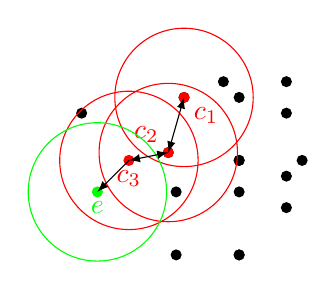
\begin{tikzpicture}
			\fill (-2,1.8) circle(2pt);
			\fill (-.9, 1.3) circle(2pt);
			\fill (-.8,.8) circle(2pt);
			\fill (-.8,0) circle(2pt);
			\fill (-.7,2) circle(2pt);
			\fill (-.2,2.2) circle(2pt);
			\fill (0,0) circle(2pt);
			\fill (0,1.2) circle(2pt);
			\fill (0,1.2) circle(2pt);
			\fill (0,0) circle(2pt);
			\fill (0,.8) circle(2pt);
			\fill (0,2) circle(2pt);
			\fill (.6,1) circle(2pt);
			\fill (.6,.6) circle(2pt);
			\fill (.6,1.8) circle(2pt);
			\fill (.6,2.2) circle(2pt);
			\fill (.8,1.2) circle(2pt);
			
			\fill[red] (-.7, 2) circle(2pt) node[anchor=north west]{$ c_1 $};
			\draw[red] (-.7, 2) circle(25pt);
			
			\fill[red] (-.9, 1.3) circle(2pt) node[anchor=south east]{$ c_2 $};
			\draw[red] (-.9, 1.3) circle(25pt);
			
			\fill[red] (-1.4,1.2) circle(2pt) node[anchor=north]{$ c_3 $};
			\draw[red] (-1.4,1.2) circle(25pt);
			
			\fill[green] (-1.8,.8) circle(2pt) node[anchor=north]{$ e $};
			\draw[green] (-1.8,.8) circle(25pt);
			
			\draw[latex-latex] (-.7, 2) -- (-.9, 1.3);
			\draw[latex-latex] (-.9, 1.3) -- (-1.4,1.2);
			\draw[-latex] (-1.4,1.2) -- (-1.8,.8);
		\end{tikzpicture}
		\subcaption{$ reach_{\varepsilon,\mu}(e, c_1) $} \label{fig:density-reachablity-reachability}
	\end{minipage}
	\begin{minipage}[b]{.5\linewidth}
		\centering
		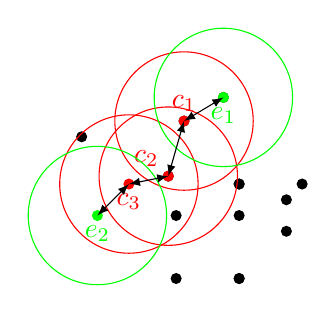
\begin{tikzpicture}
			\fill (-2,1.8) circle(2pt);
			\fill (-.9, 1.3) circle(2pt);
			\fill (-.8,.8) circle(2pt);
			\fill (-.8,0) circle(2pt);
			\fill (-.7,2) circle(2pt);
			\fill (-.2,2.3) circle(2pt);
			\fill (0,0) circle(2pt);
			\fill (0,1.2) circle(2pt);
			\fill (0,1.2) circle(2pt);
			\fill (0,0) circle(2pt);
			\fill (0,.8) circle(2pt);
			\fill (.6,1) circle(2pt);
			\fill (.6,.6) circle(2pt);
			\fill (.8,1.2) circle(2pt);
			
			\fill[red] (-.7, 2) circle(2pt) node[anchor=south]{$ c_1 $};
			\draw[red] (-.7, 2) circle(25pt);
			
			\fill[red] (-.9, 1.3) circle(2pt) node[anchor=south east]{$ c_2 $};
			\draw[red] (-.9, 1.3) circle(25pt);
			
			\fill[red] (-1.4,1.2) circle(2pt) node[anchor=north]{$ c_3 $};
			\draw[red] (-1.4,1.2) circle(25pt);
			
			\fill[green] (-1.8,.8) circle(2pt) node[anchor=north]{$ e_2 $};
			\draw[green] (-1.8,.8) circle(25pt);
			
			\fill[green] (-.2,2.3) circle(2pt) node[anchor=north]{$ e_1 $};
			\draw[green] (-.2,2.3) circle(25pt);
			
			\draw[latex-latex] (-.2,2.3) -- (-.7, 2);
			\draw[latex-latex] (-.7, 2) -- (-.9, 1.3);
			\draw[latex-latex] (-.9, 1.3) -- (-1.4,1.2);
			\draw[latex-latex] (-1.4,1.2) -- (-1.8,.8);
		\end{tikzpicture}
		\subcaption{$ connected_{\varepsilon,\mu}(e_1, e_2) $} \label{fig:density-reachablity-connection}
	\end{minipage}
	\caption{Relacje zasięgu gęstościowego \subref{fig:density-reachablity-reachability} i łączności gęstościowej \subref{fig:density-reachablity-connection}, $ \mu = 3 $.}
\end{figure}

Punkty, które nie należą do żadnej z grup nazywa się szumem. Takie punkty nie są gęstościowo połączone z żadnym innym punktem.
\begin{equation}
	noise_{\varepsilon,\mu}(p) \iff \forall i \,p\notin C_i \iff \forall q \in D \,\neg connected(p,q)
\end{equation}

\begin{algorithm}
 	\caption{DBSCAN \cite{dbscan}}\label{alg:dbscan}

	\DontPrintSemicolon
	
	\SetKwFunction{dbscan}{dbscan}
	\SetKwFunction{expand}{expandcluster}
	
	\setcounter{AlgoLine}{0}
	\nonl\SetKwProg{myproc}{Wejście}{}{}
	\myproc{}{
		$D$ - zbiór danych \;
		$\varepsilon $ - promień otoczenia \;
		$\mu $ - próg liczności otoczenia \;
	}
	\setcounter{AlgoLine}{0}
	\nonl\SetKwProg{myproc}{Wyjście}{}{}
	\myproc{}{
		każdy punkt zbioru $ D $ ma przypisaną etykietę grupy lub szumu\;
	}
	
	
	\setcounter{AlgoLine}{0}
	\nonl\SetKwProg{myproc}{Definicje}{}{}
	\myproc{}{
		$ nextcid() $ - zwraca nową unikalną etykietę grupy\;
		$ noise $ - etykieta szumu\;
		$ unde\f{}ined $ - nieokreślona etykieta\;
		$ cid(v) $ - etykieta punktu $ v $\;
		$ N_{V,\varepsilon}(v) $ - $ \varepsilon $-otoczenie punktu $ v $ w zbiorze $ V $ (\myhyperref{eps-neighbourhood}{wyrażenie})\;
		$ any(V) $ - dowolny element zbioru $ V $\;
		$ core_{V,\varepsilon,\mu}(v) $ - $ v $ jest punktem rdzeniowym w $ V $(\myhyperref{core-point}{wyrażenie})\;
	}
	\nonl\SetKwProg{myalg}{Algorytm}{}{}
	\myalg{\dbscan{$D$, $\varepsilon$, $\mu$}}{
		$ cid \gets nextcid() \;$ \tcp*{etykieta grupy}
		\ForEach{v \textbf{in} D}{
			\If{$ cid(v) = unde\f{}ined $}{
				\lIf{\expand{D, v, cid, $ \varepsilon $, $ \mu $}}{
					$ cid \gets nextcid() $
				}
			}
		}
	}
	\setcounter{AlgoLine}{0}
	\nonl\SetKwProg{myproc}{Procedura}{}{}
	\myproc{\expand{D, v, cid, $ \varepsilon $, $ \mu $}}{
		$ N_v \gets N_{D,\varepsilon}(v) $\;
		\uIf(\tcp*[f]{$ core_{D,\varepsilon,\mu}(v) $}){$ |N_v| \ge \mu $}{ 
			$ seeds \gets \set{w \in N_v | cid(w) = unde\f{}ined \land w \neq v} $\;
			\lForEach{$ w\ \mathbf{in}\ N_v $}{$ cid(w) \gets cid $}
			\While{$ seeds \neq \emptyset $} {
				$ w \gets any(seeds) $\;
				$ seeds \gets seeds \setminus \set{w} $\;
				$ N_w \gets N_{D,\varepsilon}(w) $\;
				\If($ \mathbf{foreach}\ x\ \mathbf{in}\ N_w $ \tcp*[f]{$ core_{D,\varepsilon,\mu}(w) $}){$ |N_w| \ge \mu $}{%
					\If{$ cid(x)\ \mathbf{in}\ \set{unde\f{}ined, noise} $}{
						\lIf{$ cid(x) = unde\f{}ined $}{$ seeds \gets seeds \cup \set{x} $}	
						$ cid(x) \gets cid $
					}
				}
			}
			\KwRet{true}\;
		}\Else{
			$ cid(v) \gets noise $\;
			\KwRet{false}\;
		}
	}
\end{algorithm}